\section{Personal Appendix}
\label{sec:personalAppendix}

Dieser Teil des Anhangs ist als rein informative, insbesondere pers\"onliche Erg\"anzung zu verstehen.
Er beinhaltet Hintergrundmaterial vom Autor, wie z.B. die Anlagen aus Kindheitstagen (Kap.~\ref{sec:personalAppendix_elderTracks}) oder allgemeine Inspirationsquellen f\"ur die szenische Ausgestaltung (Kap.~\ref{sec:personalAppendix_lostPlaces}.

Grafiken sind z.T. sehr klein im Dokument skaliert.
In der Ansicht am Bildschirm kann gern reingezoomt werden - qualitativ ist meistens etwas Luft nach oben vorhanden.


\subsection{Andere Anlagen im Famili\"aren oder Befreundeten Umfeld}
\label{sec:personalAppendix_elderTracks}

\textbf{Anlage Domistadt aus Kindheitstagen}

Der Gleisplan meiner in der Kindheit bespielten Anlage wurde in erster Linie von meinem Vater entworfen.
Das Abma{\ss} war $100~cm~\cdot~150~cm$.
Eine noch recht gute Ansicht ist Abb.~\ref{img:elder_maps_domistadt_map} zu entnehmen.
Dort sind bereits einige Gleise von mir zwecks Ersatzteilbereitstellung f\"ur die etwas gr\"o\"sere Anlage meines Vaters demontiert.
Es lassen sich aber durch die Aufhellungen noch gut die entfernten Gleisf\"uhrungen erkennen.
Gleiches gilt f\"ur Geb\"audeaufstellungen sowie einen Berg mit Tunnel aus Styropor, der die separierte Nebenstrecke im Oval aufwertete.

Mir hat die Anlage damals viel Freude bereitet.
Auch heute denke ich noch, dass der Gleisplan f\"ur ein Kind sehr gut durchdacht war:
\begin{enumerate}
	\item Der Au\"senbogen war mit gro\"sen Radien versehen, optimal f\"ur den ICE~1, der nebenbei tats\"achlich die erste nennenswerte Investition von meinem Ersparten war (ca. 250 DM im Fleischmann Starter-Set).
	\item Die \"Uberf\"uhrung vom Au\"sen- auf den Innenkreis stellte Gleis 2 im Bahnhof von Domistadt dar.
	\item Der Innenkreis selbst war im damaligen Neuzustand des Gleismaterials i.d.R. immer noch schnell befahrbar.
	Von ihm gehen drei Abstellgleise sowie die Kehrschleife durch das Zentrum der Platte ab.
	In der Mitte der Kehrschleife befand sich ein beschrankter Bahn\"ubergang, dessen Motor seit jeher Probleme hatte.
	\item Die ovale Nebenstrecke war ausschlie{\ss}lich f\"ur Bimmelbahnen, insbesondere mein S-Bahn Berlin Doppel-Halbzug der DR, BR ET/EB 168.
\end{enumerate}
Das Bahnhofsgeb\"aude von Vollmer, Abb.~\ref{img:elder_maps_domistadt_bhf}, ist potenzieller Kandidat zur Wiederverwertung im Bahnhof \textbf{Sch\"onblick} auf der neuen Platte Granitz.

\begin{figure}[h]
\centering
	\begin{subfigure}[b]{0.49\textwidth}
    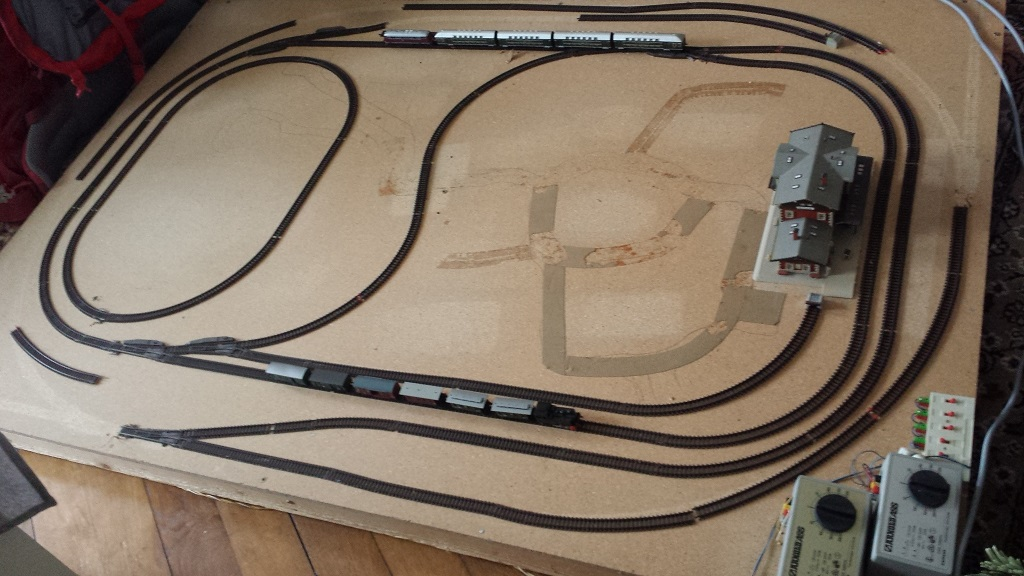
\includegraphics[width=1.0\textwidth]{img/elder_maps/domistadt_map.jpg}
   \caption{Noch erkennbarer Gleisplan der Anlage \textbf{Domistadt}}
    \label{img:elder_maps_domistadt_map}
    \end{subfigure}
	\begin{subfigure}[b]{0.49\textwidth}
    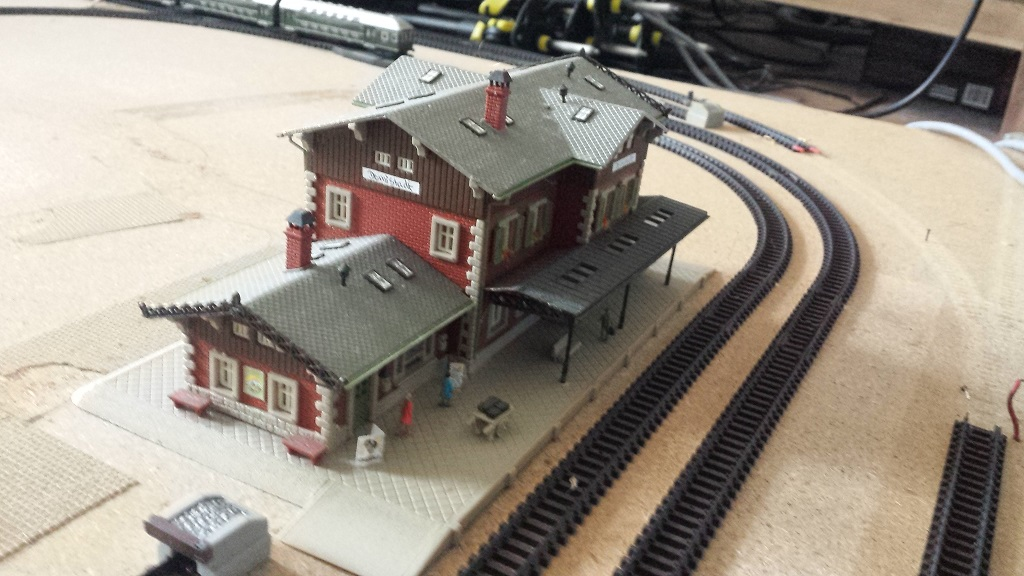
\includegraphics[width=1.0\textwidth]{img/elder_maps/domistadt_bhf.jpg}
   \caption{Hauptbahnhof von Domistadt}
    \label{img:elder_maps_domistadt_bhf}
    \end{subfigure}
		\begin{subfigure}[b]{0.49\textwidth}
    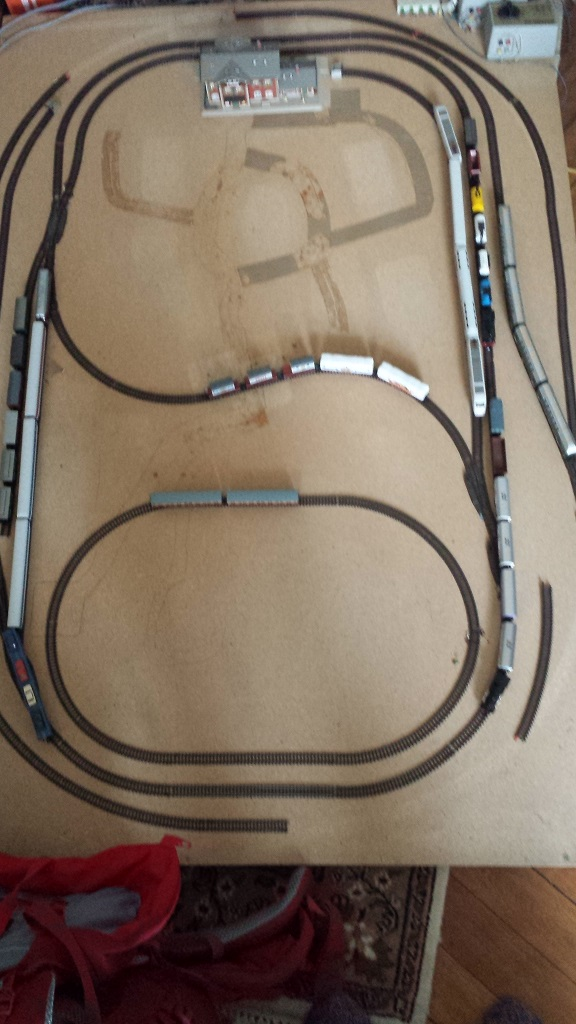
\includegraphics[width=1.0\textwidth]{img/elder_maps/train_material_childhood.jpg}
   \caption{Original Gesamtbestand Zugmaterial aus der Kindheit}
    \label{img:elder_maps_train_material_childhood}
    \end{subfigure}
		\begin{subfigure}[b]{0.49\textwidth}
    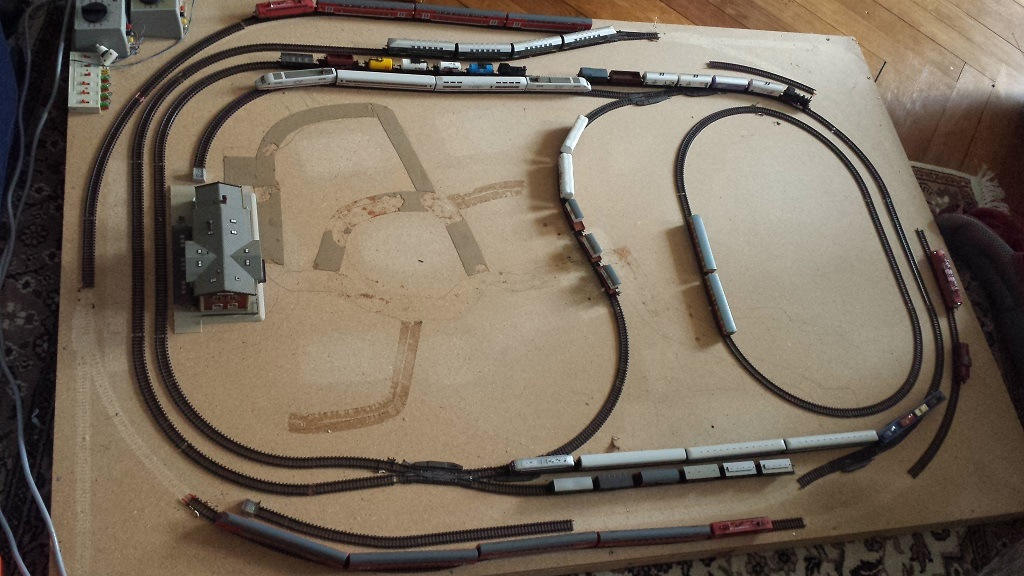
\includegraphics[width=1.0\textwidth]{img/elder_maps/train_material_kickoff.jpg}
   \caption{Erweiterter Gesamtbestand Zugmaterial zum Kick-Off von Granitz, Februar 2020}
    \label{img:elder_maps_train_material_kickoff}
    \end{subfigure}
	\caption{Meine Anlage aus Kindheitstagen in z.T. r\"uckgebautem Zustand}
	\label{img:elder_maps_domistadt}
\end{figure}

Der Zugmaterialbestand aus der Kindheit erwies sich bei der Inventur Anfang 2020 als gute Basis.
Er ist auf den Resten der Anlage Domistadt aufgestellt in Abb.~\ref{img:elder_maps_train_material_childhood} zu sehen.
Neben einigen Epoche V Schnellz\"ugen, dem dunkelgr\"unen Sputnik und der BR 217 sind auch \"altere Jahrg\"ange vertreten.
Die aktionistische Aufstockung Anfang 2020 zum Kick-Off der Arbeiten an Granitz sind zus\"atzlich in Abb.~\ref{img:elder_maps_train_material_kickoff} abgebildet.

Direkt nach Abfotografieren der alten und zum Kick-Off aktuellen Flotte wurde die Anlage Domistadt vollst\"andig zur\"uckgebaut.
Die Trafos sowie die noch brauchbare Gleise finden im neuen Szenario Wiederverwertung.
Noch viel wichtiger: Die Spanplatte ist nun das zentrale Segment vom Granitzer Nordriegel.
Der Geist von Domistadt geht damit nicht vollst\"andig verloren, die alten Gleis- und H\"auserschatten bleiben sicherlich ebenso noch irgendwo im Verborgenen erhalten.


\textbf{Anlage meines Vaters, damals \"ahnlich heute}

Ein Foto der Platte meines Vaters - so ist sie gegenw\"artig nach geringf\"ugigen Modifikationen wieder bespielbar - wurde bereits in der Einleitung, Abb.~\ref{img:elder_maps_anlage_papa_2019} gezeigt.
Die Abmessung ist in der L\"ange etwas gr\"o{\ss}er als die von Domistadt, n\"amlich $100~cm~\cdot~180~cm$.
Ein per Hand aufgel\"oster Gleisplan ist Abb.~\ref{img:elder_maps_anlage_papa_map_domi} zu entnehmen.

\begin{figure}[h]
\centering
  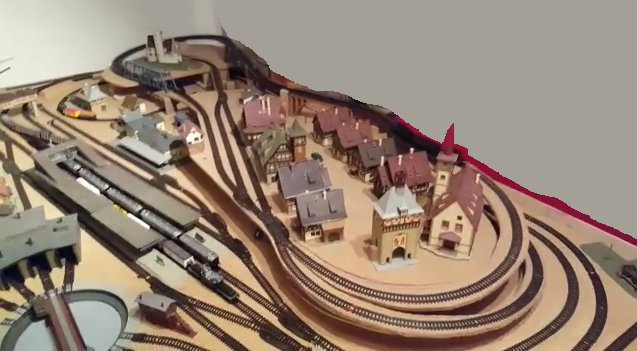
\includegraphics[width=0.5\textwidth]{img/elder_maps/anlage_papa_2019.png}
	\caption{Skizze des Gleisplans mit verschiedenen Schaltkreisen\hl{ ; ABBILDUNG AUSZUTAUSCHEN!}}
	\label{img:elder_maps_anlage_papa_map_domi}
\end{figure}

Wiederum ist die Hauptstrecke ein Oval.
Der Hauptbahnhof f\"ur den Personenverkehr ist viergleisig und bedient dabei jede Fahrtrichtung mit einem Bahnsteig.
Die Bahnsteigl\"ange ist \hl{$XX~cm$}, so dass hier schon ann\"ahernd vern\"unftige Z\"uge mit ca. vier Personenwaggons Platz \"uber die L\"ange finden.
An der S\"udseite des Bahnhofs, dort ist auch das relativ schlichte Empfangsgeb\"aude gelegen, findet sich ein Rangiebereich inlusive zwei Lokschuppen mit Drehscheibe.

Der zentrale Berg bildet Schauplatz f\"ur zwei eingleisige Nebenstrecken:
\begin{enumerate}
	\item Die erste f\"uhrt von der nordwestlichen Bahnhofsausfahrt auf den im Berg und h\"alt im Bahnhof des Bergortes.
	\item Sie wird sodann wieder Richtung S\"udost den Berg hinuntergef\"uhrt, agiert somit als Wendeschleife und wird jenseits des Bergs auf die Hauptstrecke zur\"uckgef\"uhrt.
	Direkt im Anschluss befindet sich auch ein Gleiswechsel der Hauptstrecke.
	\item Die zweite Nebenstrecke befindet sich auf dem Berg selbst und ist vorwiegend als langgezogene, ovalf\"ormige Hochbahn ausgef\"uhrt.
	Ihr einziger Halt ist im Bahnhof des Bergortes, wo eine \"Uberf\"uhrung auf die erste Nebenstrecke erfolgen kann.
	\item Die Crux gerade dieser Hochbahn ist ihre leider viel zu starke Steigung sowie die etwas fragile Hochbahnkonstruktion, bedingt durch die Vorgabe, die Br\"uckenelemente unbedingt zu erhalten.
\end{enumerate}

Ein paar Defizite hinsichtlich des spielerischen Betriebs wurden um Weihnachten 2018 und 2019 herum ausgem\"arzt.
Insgesamt w\"urde ich die Anlage so niemals bauen, aber sie ist in meinen Augen okay.

Ein gro\"ser Unterschied zu Granitz ist ganz einfach der, dass diese Anlage auf begrenztem Platz viel anbietet, dadurch aber nat\"urlich von der Realit\"at deutlich abweichen muss.
Eine detaillierte Dioramaausgestaltung fehlt leider bis heute, was ihre Attraktivit\"at noch mal ungemein steigern w\"urde.
Dem m\"ochte ich mich in der Zukunft gern noch mal annehmen.
Aktuell ist die Zukunft der Platte aber aus mehreren Gr\"unden ungewiss; mitunter fehlt mir durch das Granitzprojekt nat\"urlich auch die Zeit.
Die Hoffnung besteht aber, dass meine Erfahrungen beim Bau von Granitz hier relativ schnell umzusetzende L\"osungen bzgl. szenischer Ausgestaltung beitragen werden.

\textbf{Anlage meines Bruders}

Die Abma{\ss}e der Platte meines Bruders waren mit der von Domistadt identisch.
Der Gleisplan ist mir leider nur geringf\"ugig in Erinnerung:
\begin{itemize}
	\item doppelgleisige Hauptstrecke im Oval
	\item achtf\"ormige, zentral verortete Bimmelbahnstrecke
	\item der mehrgleisige Bahnhof (meiner Erinnerung nach Teile des Bonner Bahnhofs von Faller) hatte benachbart einige Abstellgleise
	\item in dunkler Erinnerung habe ich eine etwa zentral verlaufende Verbindungsstrecke zwischen der Nord- und S\"udseite des Ovals
\end{itemize}
Ggf. kann mir mein Bruder hier eines Tages aushelfen.

\textbf{Anlage meiner Mutter}

Die Aktivit\"at meiner Mutter auf der Modelleisenbahn war wahrscheinlich eher uns Kindern gewidmet.
Ihre Anlage war - so w\"urde ich es heute bezeichnen - rein obligatorisch:
Ein verkleinerter Quadratgrundriss mit ca. $75~cm$ Kantenl\"ange mit einem spiralartigen Gleisplan.

\textbf{Der Inter-Famili\"are Zusammenschluss}

Zu den Hochzeiten gab es einen Kellerraum, der allein diesen vier Platten und ihrem Zusammenschluss gewidmet war.
Das entsprechende Setup ist in Abb.~\ref{img:elder_maps_keller_TA8} dargestellt.
Die Hauptstrecken sind angedeutet sowie die Lage der bekannten Hauptbahnh\"ofe durch schwarze Rechtecke verzeichnet.
Wandseitig gab es eingleisige \"Uberf\"uhrungsstrecken.
Der Zusammenschluss zwischen Domistadt und der Platte meiner Mutter hatte hinter der Anlagenkante noch etwas Platz, so dass mein Steuerpult tats\"achlich direkt vor meinem Hauptbahnhof platziert war.

Das besondere war nat\"urlich, dass prinzipiell die Anlagen aller als Segmente befahren werden konnten.
Mir war die Anlage meines Vaters aber aufgrund ihrer h\"oheren Komplexit\"at verboten - ein paar mal habe ich es trotzdem geheim probiert - und mein Bruder war aus irrationalen Gr\"unden (xD) noch viel restriktiver im Freigabeprozedere.
Zur benachbarten 'Mutterplatte' gab es aber regen Austausch.

\begin{figure}[h]
\centering
  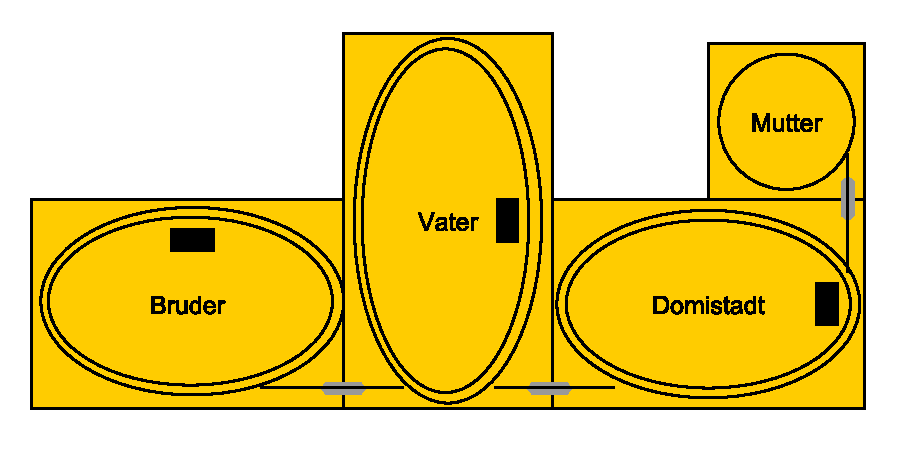
\includegraphics[width=0.5\textwidth]{img/elder_maps/keller_TA8.pdf}
	\caption{Skizze des Zusammenschlusses aller vier Platten}
	\label{img:elder_maps_keller_TA8}
\end{figure}




\subsection{Lost Places und Andere Inspirationsquellen (Fotosammlung)}
\label{sec:personalAppendix_lostPlaces}

\textbf{Ehemalige Kaserne Vogelsang}


\textbf{Flughafen Gro{\ss}-D\"olln}


\textbf{Lieberoser W\"uste}


\textbf{Bahnhof Werneuchen}


\textbf{Stillgelegter Haltepunkt Bahnhof Grieben}


\textbf{Gegen\"uber vom Westhafen Berlin}

Am Nordende von Berlin-Moabit liegt der Westhafen.
Zu Zeiten der Deutschen Teilung ein extrem wichtiger Umschlagplatz f\"ur Westberlin, hat er heute immer noch Bedeutung.
Am S-Bahn Ring befindet sich zwischen den S-Bahnh\"ofen Beusselstra{\ss}e und Westhafen (Kreuzungspunkt mit der U-Bahn-Linie 9) ein inzwischen weitestgehend zur\"uckgebautes G\"uterbahnhofsgel\"ande.
Immernoch ist die Trasse sehr breit:
\begin{itemize}
	\item Ganz im Norden befinden sich die Gleise vom Umschlag am Westbahnhof, die immer noch von der BeHaLa in Nutzung sind.
	\item Noch im n\"ordlichen Bereich der Beusselstra{\ss}en-Br\"ucke sowie Putlitzbr\"ucke gelegen, befindet sich die doppelgleisige Berliner Ringbahn.
	\item Es folgen einige Gleise, die f\"ur den Regional- und Fernverkehr genutzt werden, der zwischen dem westlich gelegenen Bahnhof Jungfernheide (dahinter Gabelung nach Spandau bzw. Westkreuz) und dem \"ostlich gelegenen Hauptbahnhof abgewickelt wird.
	\item Die s\"udlichen Gleise sind Betriebsgleise, auf denen zumeist G\"uterz\"uge und Regios, aber hin und wieder auch mal ein ICE zwischengeparkt werden.
\end{itemize}
Zusammengefasst muss man eingestehen: Die beiden Br\"ucken bieten eine spannende und relativ bunte \"Ubersicht zu wesentlichen Zugverbindungen von und nach Berlin.

Wie weit sich der G\"uterbahnhof damals an das Wohngebiet anschmiegte, ist auf alten Pl\"anen noch gut zu sehen.
Etliche weitere Gleise wurden abgerissen:
\begin{itemize}
	\item Direkt s\"udlich der verbliebenen Trasse schmiegt sich heute die ziemlich h\"assliche Umgehungsstra{\ss}e (Erna-Samuel-Stra{\ss}e) an.
	\item Ein altes Geb\"aude mit Rampe bildet heute das Zentrum des Stadgartens, auch ZK/U genannt.
	Hier haben ein paar K\"unstler Platz f\"ur kreatives Schaffen gefunden und das ist auch gut so.
	Die kleine Gr\"unanlage rund um das Geb\"aude ist bei den Moabitern und auch mir ein recht beliebter Verweilort.
	\item Wenn man seinen Spaziergang \"uber die Putlitzbr\"ucke hinaus nach Osten verl\"angert, dann sieht man an den R\"andern der Grundst\"ucke des heutigen Gewerbegebiets (Supermarkt, Baumarkt etc.) auch noch das begrenzende, nat\"urlich l\"angst ungenutzt Gleis hinter den Z\"aunen.
	Dort gegen\"uber befindet sich dann auch schon das Kraftwerk Moabit.
\end{itemize}

Das gesamte Areal k\"onnte eigentlich auch dem feuchten Traum eines Modellbahners sein, der viel Platz zu Hause hat.
Die Kombination aus Hafen und Kraftwerk auf der einen Seite, dem fetten Gleisriegel im Zentrum, den R\"uckbauten im S\"uden und das schlussendlich angrenzende Berliner Wohngebiet mitsamt Altbauten ist aber durchaus Realit\"at.

Hier ein paar Eindr\"ucke:

\begin{figure}[h]
\centering
	\begin{subfigure}[b]{0.49\textwidth}
    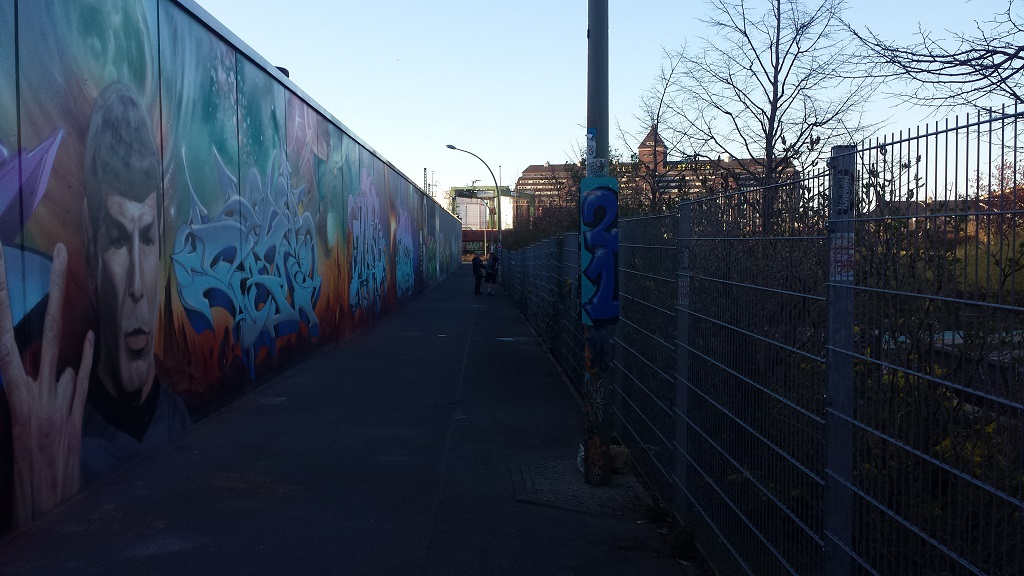
\includegraphics[width=1.0\textwidth]{img/inspiration/westhafen_view_preDurchgang.jpg}
   \caption{Fu{\ss}g\"angerdurchgang zwischen einem Gro{\ss}handel und dem Stadtgarten am ZK/U, links eine freigegebene Graffitifl\"ache, geradeaus der Westhafen mit vorgelagerter Bahntrasse}
    \label{img:inspiration_westhafen_view_preDurchgang}
    \end{subfigure}
	\begin{subfigure}[b]{0.49\textwidth}
    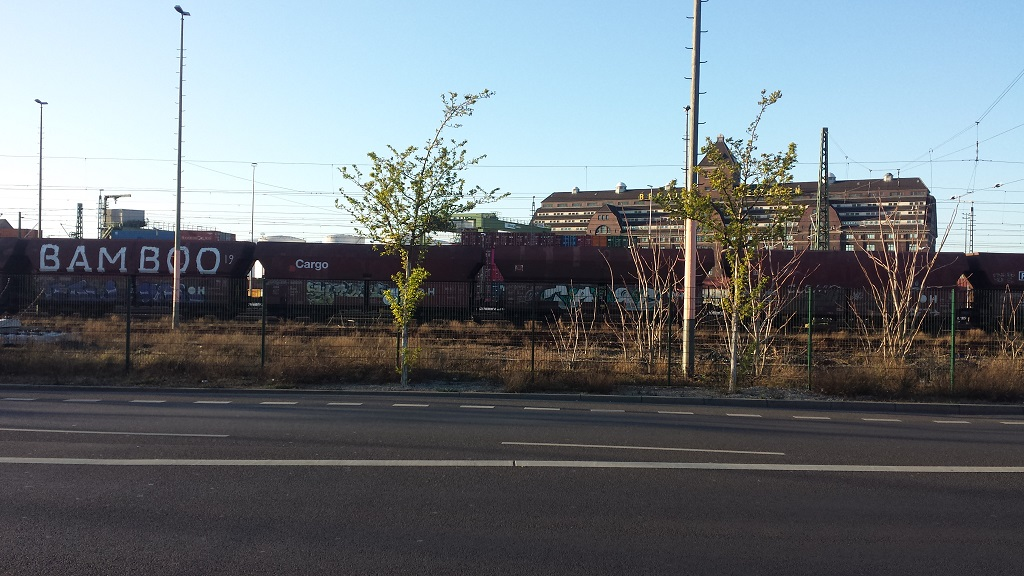
\includegraphics[width=1.0\textwidth]{img/inspiration/westhafen_view_postDurchgang.jpg}
   \caption{Am Ende des Fu{\ss}g\"angerdurchgangs: typisch abgeranzte Hinterbahnhofshalde mit abgestelltem Lorenzug, irgendwer hat sich daran verewigt, aber niemanden interessiert es}
    \label{img:inspiration_westhafen_view_postDurchgang}
    \end{subfigure}
	\caption{Fu{\ss}g\"angerdurchgang am Stadtgarten des ZK/U Gel\"andes}
	\label{img:inspiration_westhafen_view_durchgang}
\end{figure}



\textbf{U-Bahn-Linie 9 der BVG}

Die U9 hat mein Leben beinahe zu jederzeit begleitet - oder ich sie.
Der architektonische Stil der Bahnh\"ofe ist h\"aufig 60er/70er Jahre gepr\"agt.
Insbesondere die Bahnh\"ofe in Berlin-Steglitz sind recht 'poppig'.
Hier einfach mal ein paar Fotos:

\textit{ToIntegrate}

